\section{Технологическая часть}

\subsection{Выбор и обоснование языка программирования и среды разработки}

Для реализации разработанного метода используется язык программирования Kotlin – статически типизированный, объектно-ориентированный язык программирования\cite{Kotlin}, поскольку имеется опыт ведения разработки на данном языке, что сократит время кодирования программы. 

Ключевой особенностью языка Kotlin является то, что его код сначала транслируется в специальный байт-код, независимый от платформы. А затем этот байт-код выполняется виртуальной машиной JVM (Java Virtual Machine). В этом плане Java отличается от стандартных интерпретируемых языков, код которых сразу же выполняется интерпретатором. В то же время Kotlin не является и чисто компилируемым языком.

Подобная архитектура обеспечивает кроссплатформенность и аппаратную переносимость программ, благодаря чему подобные программы без перекомпиляции могут выполняться на различных платформах - Windows, Linux, Mac OS и т.д. Для каждой из платформ может быть своя реализация виртуальной машины JVM, но каждая из них может выполнять один и тот же код.

В качестве среды разработки была выбрана одна из самых популярных – IntelliJ IDEA от компании JetBrains\cite{idea}.

Среди преимуществ данной программы можно выделить следующие:

\begin{itemize}[leftmargin=1.6\parindent]
	\item[---] наличие студенческой лицензии для ведения некоммерческой разработки;
	\item[---] простые и удобные средства отладки программного кода;
	\item[---] интеграция с системой контроля версий;
	\item[---] работа с базой данных, получение выгрузок и резервных копий;
	\item[---] встроенные средства автоматизации сборки проекта.
	
\end{itemize}

Для реализации фронтенд части проекта был использован JavaScript – один из самых популярных языков программирования в мире. Он используется для создания интерактивных веб-страниц.

\subsection{Организация клиент-серверного взаимодействия}

Поскольку для взаимодействия с конечным пользователем было решено использовать веб-интерфейс, который предусматривает дальнейшее расширение и масштабирование приложения, необходимо организовать передачу сообщений от сервера к клиенту в реальном времени без перезагрузки страницы. 

Для решения данной задачи была выбрана технология Server-Send Events (SSE)\cite{sse}. Основная концепция заключается в том, что клиент подписывается на события, присылаемые сервером, в свою очередь сервер шлет их с помощью специального объекта, который именуется как SSE Emitter. На рисунке \ref{sse} показан пример такого взаимодействия.

\begin{figure}[hbtp]
	\centering
	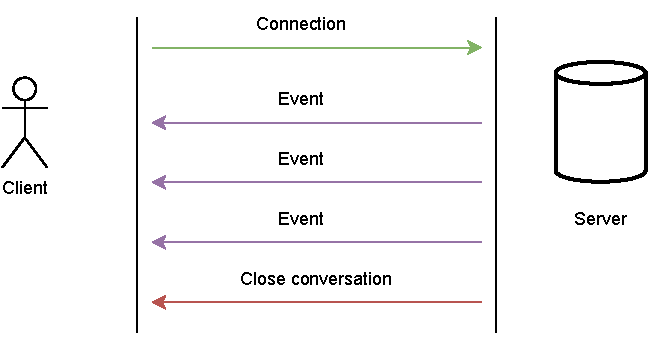
\includegraphics[scale=1.1]{img/sse.drawio.pdf}
	\caption{Организация взаимодействия по технологии SSE}
	\label{sse}
\end{figure}

\subsection{Структура разработанного ПО}

Структура разработанного программного обеспечения представлена на рисунке \ref{developed}.

\begin{figure}[hbtp]
	\centering
	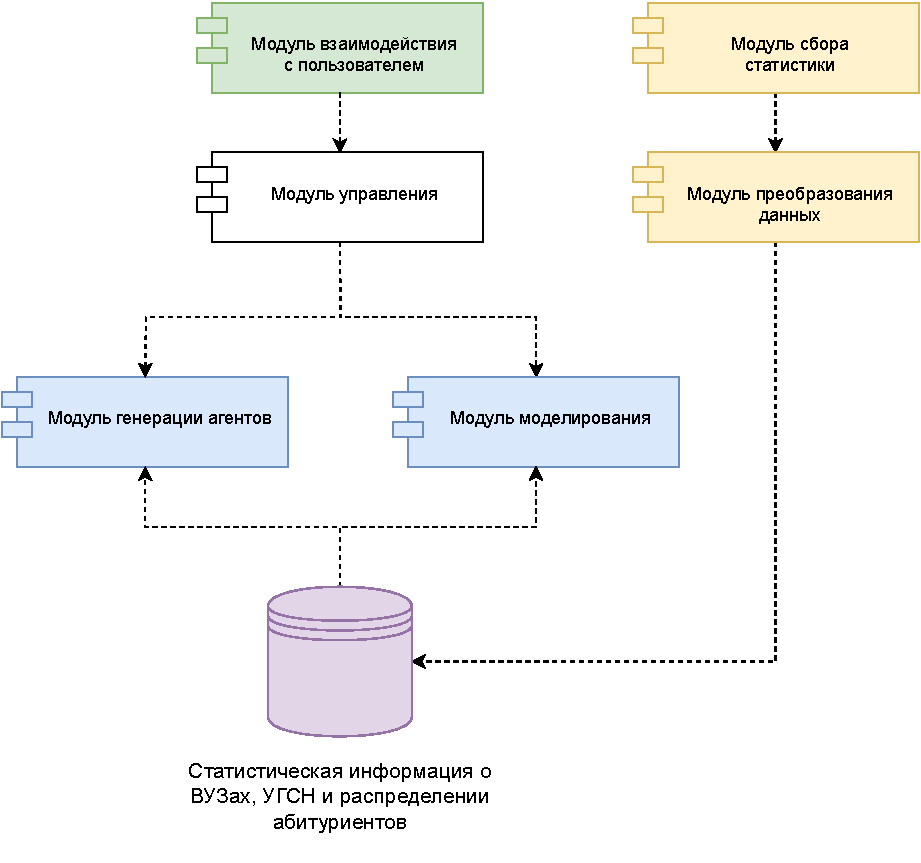
\includegraphics[scale=1.1]{img/developed.drawio.pdf}
	\caption{Структура программного обеспечения}
	\label{developed}
\end{figure}

Каждый модуль, изображенный на диаграмме, содержит в себе
сгруппированные по функциональному значению соответствующие классы.
Модуль взаимодействия с пользователем отвечает за пользовательский
интерфейс. Модуль управления связывает модули разработанного метода и модуль взаимодействия с пользователем. 

Отвечающие за сбор и обработку информации модули напрямую взаимодействуют с энергонезависимым хранилищем информации для сохранения и дальнейшего переиспользования другими модулями.

\subsection{Минимальные требования к вычислительной системе}

Для того, чтобы воспользоваться программным продуктом, достаточно только ЭВМ, на которой будет установлена JRE (Java Runtime Environment) — минимальная реализация виртуальной машины, необходимая для исполнения Kotlin-приложений, без компилятора и других средств разработки.

Минимальные требования к вычислительной системе:

\begin{itemize}[leftmargin=1.6\parindent]
	\item[---] операционная система Windows 7 или младше, Ubuntu 16.04, MacOS Monterey 12.0.1;
	\item[---] оперативная память – 8 Гб.
	
\end{itemize}

При указанных выше параметрах программный продукт будет штатно функционировать.

\subsection{Формат входных и выходных данных}

Входными данными для генерации агентов являются:

\begin{itemize}[leftmargin=1.6\parindent]
	\item[---] процентные соотношения численности категорий студентов с различными диапазонами полученных результатов ЕГЭ;
	\item[---] диапазон результатов ЕГЭ, которые будут заданы агентам каждой категории;
	\item[---] процентные соотношения признака смены региона для каждой категории;
	\item[---] количество различных УГСН, которые рассматривает агент;
	\item[---] минимальные баллы ЕГЭ по каждому предмету.
\end{itemize}

Входными данными для процесса моделирования являются:

\begin{itemize}[leftmargin=1.6\parindent]
	\item[---] год проведения моделирования;
	\item[---] количество абитуриентов, участвующих в моделировании;
	\item[---] длительность этапа перераспределения заявлений с копиями аттестатов;
	\item[---] максимальное количество ВУЗов, в которое может подать заявления агент;
	\item[---] длительность этапа поиска наилучшего места для оригинала аттестата.
	
\end{itemize}

Выходными данными является список строк формата: именование университета, полученный в ходе моделирования средний балл по ВУЗу, средний балл прошлого года, изменение среднего балла по сравнению с прошлым годом, минимальный балл, максимальный балл, количество поступивших абитуриентов. А также связанные с данным ВУЗом результаты каждого УГСН в формате: именование УГСН, полученный в ходе моделирования средний балл по УГСН,, средний балл прошлого года, изменение среднего балла по сравнению с прошлым годом, минимальный балл, максимальный балл, количество поступивших абитуриентов.


\subsection{Тестирование ПО}

Адекватность реализованного метода проверялась путем проведения моделирования на статистических данных ВУЗов и УГСН за 2020 год и сравнения с результатами приемной кампании того же года. На рисунке \ref{top5tech} представлены результаты тестирования для выборки технических ВУЗов. Результаты работы с разбиением по медицинским и гуманитарным категориям представлены на рисунках ниже.

\begin{figure}[hbtp]
	\centering
	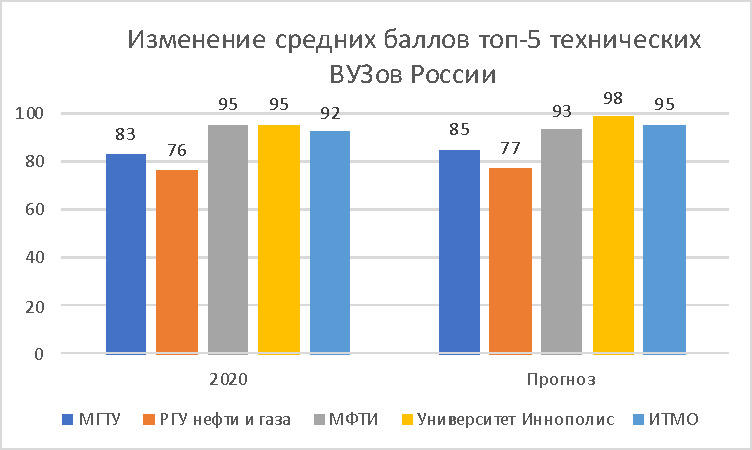
\includegraphics[scale=1.1]{img/top5tech.pdf.pdf}
	\caption{Изменение средних баллов ТОП-5 технических ВУЗов}
	\label{top5tech}
\end{figure} 

\begin{figure}[hbtp]
	\centering
	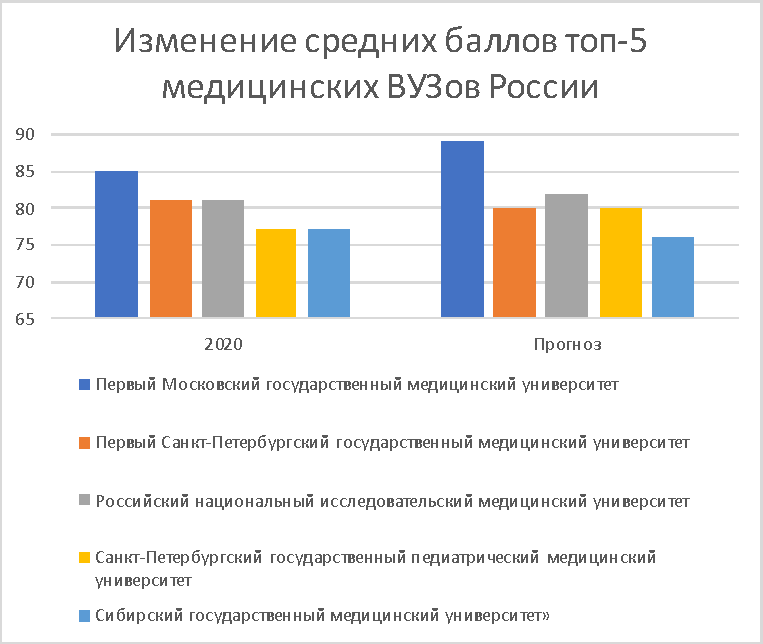
\includegraphics[scale=1.1]{img/top5med.pdf.pdf}
	\caption{Изменение средних баллов ТОП-5 медицинских ВУЗов}
	\label{top5tech}
\end{figure} 

\begin{figure}[hbtp]
	\centering
	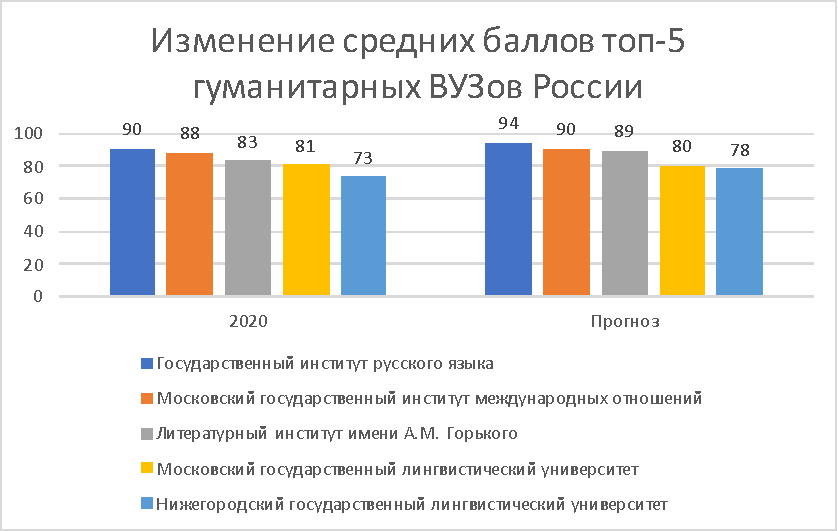
\includegraphics[scale=1.1]{img/top5gym.pdf.pdf}
	\caption{Изменение средних баллов ТОП-5 гуманитарных ВУЗов}
	\label{top5tech}
\end{figure} 	

На рисунках видно боковую динамику, резких изменений среднего балла не наблюдается.

\pagebreak